\section{Research methods}

% This chapter, as well as the next one, will be divided into two main sections, the first describing the system development and the second the system evaluation.

\subsection{System development}

In this section I will explain the rational for the choises of system implementation in the context of the above research targets.

\subsubsection{Mobile and Android}

% Deciding to go mobile, including all the information from the literature review about the growth of social use of mobile devices etc.

Recent studies state that today's mobile phone ``has become such an important aspect of a user's daily life that it has moved from being a mere `technological object' to a key `social object{'}''\todo{rephraze, don't cite}, and as such it has a significant importance in shaping today's society (\cite{srivastava05}).
This research is targeted for the general audiance and therefor will be implemented for mobile.

The system will be developed for the Android operation system (``\citetitle{web:android}'').
Choosing Android as the platform for my research has two main advantages:
\begin{enumerate}
	\item The Android system is a growing mobile system which controls most of the market share today (``\citetitle{wiki:mobile}''\todo{DON'T CITE WIKIPEDIA or ``see www.wikipedia.com/...'' in the footnote}).
	\item By developing application for Android I have access to underlying Bluetooth properties such as received signal strength indicator (RSSI), which is essential for my implementation of the system as laid out in the next section.
\end{enumerate}

\subsubsection{Indoor positioning system}\label{methods:ips}

% Explain why I've decided to implement my own indoor positioning system. For HCI it was a good idea to push it to the front, for BI music department I'm not so sure...

Although there are available techniques to implement IPS I have decided to develop one by my own.
This decision have been done due to two reasons:
\begin{enumerate}
	\item The above techniques, as well as most of their alternatives, require infrastructure.
	As a system influenced by flash mobs I wanted to be able to use it anywhere without the effort involved in infrastructure deployment.
	\item Tracking the positioning of the participants as well as the positioning of the balloon bundles has a lot of overhead when the only requirement is to be able to approximate the distance between each participant and the bundles.
	\item As opposed to system where high accuracy is required, in the current reseach does not demend it.
	Being able to estimate if a participant is `close' to a beacon or far from it is generaly satisfying.
\end{enumerate}

% the BBRIP system

The system I've developed -- the Bluetooth Based Relative Indoor Positioning (BBRIP) system -- is a distributed system that runs separately on each one of the participants phones.
The system consist of some Bluetooth beacons, placed inside the balloon bundles, and an Android application.
The application repeatedly searches for nearby Bluetooth beacons.
Received signal strength indication (RSSI) is used as an estimation of the distance between the user and the beacon.

\subsubsection{libpd}\label{methods:libpd}

Advance audio processing is beyond the capabilities of the Android application programming interface (API) and therefor, in order to apply sophisticate manipulations on the audio in real time, a more powerful audio engine was required.
In a personal computer environment the programming language Pure Data (Pd), originally written by Miller Puckette in the nineteen-nineties, is one of the leading open-source softwares for computer music (\cite{web:pd}).
In this research I have decided to use ``libpd'', a thin layer on top of Pd that turns it into an embeddable audio library, as an audio engine (\cite[page v]{brinkmann12}).

\subsubsection{System description}\label{systemdescription}

\todo{enhance and make this subsection simpler}

From the participants point of view the system will consist of few balloon bundles, each one corresponds to a specific musical style.
When the participants will stroll between the balloon bundles with their mobile devices and headphones their relative distances from the different bundles will affect the music in their headphones, creating virtual ``sound zones'' around each balloon bundle.
The distance between each participant and sound zones may affect the music in several different ways.
For example, when a participant get close to specific sound zone the music filtration may change according to the distance.
For another sound zone the volume may be changed when getting close to it or walk away.
Although the style of each sound zone will be well-definition, every sound zone will by able to be heard with any other sound zone, in synchronization and harmony.
In addition, participants will be able to freely move the balloon bundles, thereby changing the structure of the music in the virtual space\footnote{A video demonstrating the system behavior from the participant point of view can be found at \href{http://youtu.be/2kJoeD2iWBA}{youtu.be/2kJoeD2iWBA}.}.

\begin{figure}[h]
	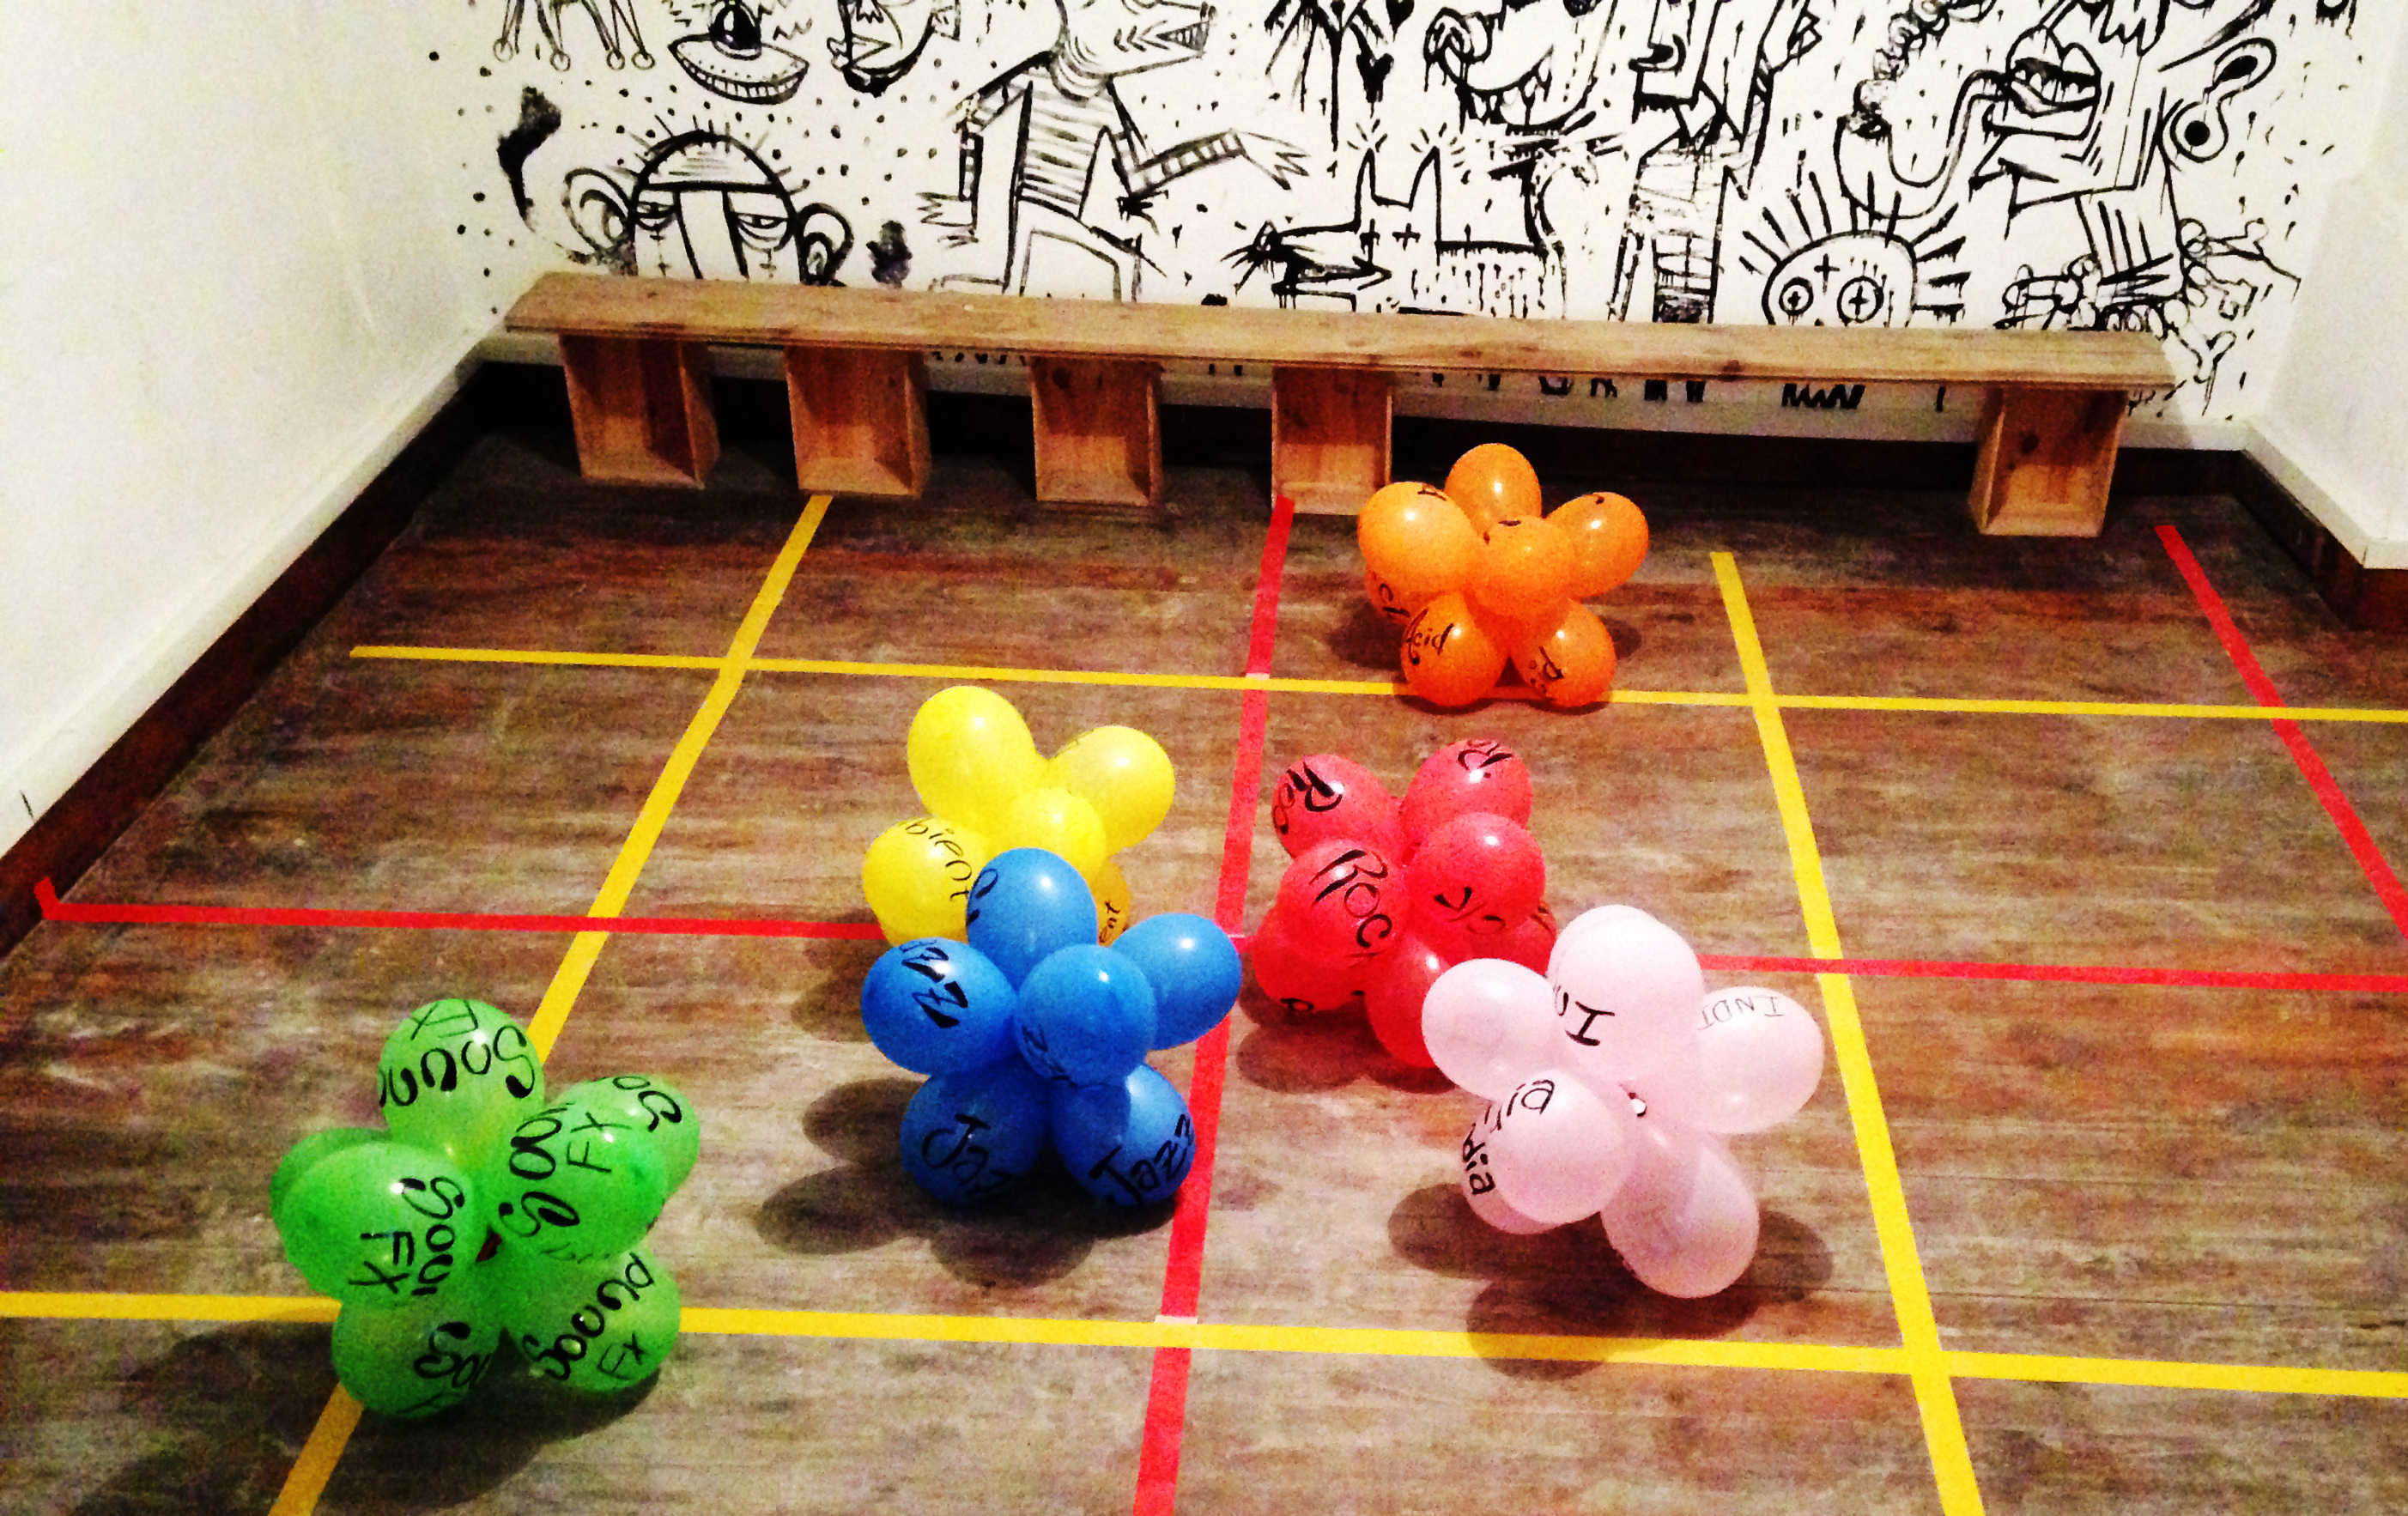
\includegraphics[width=\linewidth]{balloons}
	\caption{Balloon bundles on the dance floor}
\end{figure}

\subsection{System evaluation}\label{methods:evaluation}

% The following, as described in the meeting summary.
A controlled experiment will be conducted in order to asses the research question: \emph{Does the system elaborate social interaction between participants in an interactive silent disco party?}

\subsubsection{Participants}

Thirty undergraduate and graduate-level students from the Music Department of Bar-Ilan university will participate in the experiment.
Their participation will rely on voluntarily will.\todo{anything else?}

\subsubsection{Measurements}

The above research question will be fragmented into the following operational definitions and measurements\footnote{Complete version of each of the surveys below can be found in the appendix.}:
\begin{enumerate}
	\item \label{measure:disperse} Assuming that participants are pre-partitioned, natively, as groups of friends, we can define the \definition{momentary center} of each group as the average positioning of its participants on the two dimensional plain of the dance floor.
	In addition, we can define the \definition{momentary disperse} of each group as the variance of its participant's positionings around the center.
	Using the above definitions interaction between the members of one group with other participants will be evaluated by the disperse of the groups, when high disperse values indicate higher interactivity.
	\item \label{measure:groups} Using the above definitions, we can define \definition{momentary group disperse} as the variance of the momentary centers themselves on the dance floor.
	With this regards low momentary group disperse values indicate higher interactivity.
	\item \label{measure:audio} The audio volume inside the experiment room will be used as an indication for the amount of `speaking' between participants and therefor as a social interaction estimation.
	\item \label{measure:survey:social} Participants will fill social interaction survey\todo{write it!}.
	The survey will be used to asses interaction between participants by estimating social cohesiveness within in-group and out-group of each participant (\todo{find ref}).
\end{enumerate}
In addition to measurements intended to assess the main research question.
The following operational definitions and measurements will be used in order to assess interaction with and satisfaction from the system.
\begin{enumerate}[resume]
	\item \label{measure:system} We will define \definition{momentary participant-system interaction} as the momentary distance of each participant from the closest Bluetooth beacon.
	Using the above definition high level of interaction of participant with the system will be indicated by low values of momentary participant-system interaction.
	\item \label{measure:survey:usability} Participants will fill system satisfaction survey, based on the System Usability Scale (\cite{brooke96}).
\end{enumerate}
Lastly, the following measurement will be used in order to eliminate possible differences between research groups and to allow future research based on the retrieved data.
\begin{enumerate}[resume]
	\item \label{measure:survey:musical} Participants will fill musical background survey, based on the Emmanuel College Music Background Questionnaire, basic version (\cite{web:zhao12}).
\end{enumerate}

\subsubsection{Apparatus}

In order to measure momentary disperse and group disperse as defined in measurements \ref{measure:disperse} and \ref{measure:groups} I will capture the experiment with video camera from above the dance floor.
Tracking the positioning of the participants will be done half manually by using software aids to record the manual tracking of participants, each at a time, using the computer mouse.
The results will be then processed using computational programming to conclude insights from the data.
Tracking data required in order to compute momentary participant-system interaction, as described in measurement \ref{measure:system}, will be derived the same way, by manually tracking each on of the system components in the video.

Audio volume (measurement \ref{measure:audio}) will be captured by a microphone and analyzed afterwards.

\subsubsection{Procedure}

Participants will be randomly allocated into two groups, group $A$ and group $B$\@.
Each group will participate in the experiment in different week, but in the same day of the week and same hour.

\begin{figure}[!hb]
	\centering
	\def\svgwidth{0.8\textwidth}
  	\input{graphics/procedure.pdf_tex}
	\caption{Experiment design}\label{fig:experiment}
\end{figure}

For each group, participants will first fill a musical background survey as described in measurement \ref{measure:survey:musical}, followed by three \definition{experiment blocks}, followed by a system usability survey as described in measurement \ref{measure:survey:usability} (see figure \ref{fig:experiment}.
Each experiment block will consist of 15 minutes in which participants listen to music in their headphones, using their Android device and pre-installed application, and interact with other participants in the `silent disco' party.
Meanwhile, during each experiment block, measurements \ref{measure:disperse}, \ref{measure:groups}, \ref{measure:audio} and \ref{measure:system} will be collected.
Before each experiment block and after the last block each participant will fill the social interaction survey (measurement \ref{measure:survey:social}).

Each experiment block can be of one of the following types:
\begin{description}
	\item[Interactive:] In which the music generated by the Android application behaves as described in chapter \ref{roadmap}.
	\item[Control:] In which the music generated by the Android application is pre-composed and based on the same musical materials as of the interactive system.
\end{description}

Participants of group $A$ will hear the experiment blocks: Control $\rightarrow$ Interactive $\rightarrow$ Control. Whereas participants of group $B$ will hear the experiment blocks: Control $\rightarrow$ Control $\rightarrow$ Control.
